\documentclass{article}
%\usepackage[utf8]{inputenc}
\usepackage{hyperref}
\usepackage{graphicx}
\usepackage{float}
%\usepackage{listings}

\title{Assignement 5}
\author{Iván Piña Arévalo \\ ivan.pinaarevalo@alum.uca.es}
\date{\today}

\begin{document}
\maketitle

\newpage
\begin{abstract}
    In this practice we will make an approximation of Travelling Salesman Problem (TSP). 
    This problem is well known as NP-Hard, so finding an optimal solution in polinomial time is not possible in the present 
    day. For the approximation we have utilized a genetic approach. We use two different crossover operators, analysing the 
    result of each one of them. Likewise we supply to the program of an important randomness factor for increasing the space 
    with of the explored states.
\end{abstract}

\newpage
\section{Introduction}
We will begin speaking of the travelling Salesman Problem. It consists of a cities set, to find the cities sequence such that 
the traveled distance is the minimum, beginning from an origin and ending in the same origin. As we can see, according to the 
cities number is increasing, a boom of possible combinations happens. This is why a brute force approach is not appropiate.
Instead of finding the optimal solution, we can use computable algorithms that provide an optimal solution approachment. In 
other words, it is not the best solution, but it is sufficiently enough.


we can use two algorithms set in order to achieve the approach:
    \begin{itemize}
        \item Ant Colony Optimisation: It is based on the procedure that ants use to find the shortest route between their 
        colony and possible meats. In broad terms we could say that each worker ant is leaving pheromones in their path. 
        Consecuently, the shortest route will have more pheromones that the rest of routes (we make it in less time). The other
        ants choose the path that have more pheromones (they deducte it is more short and safe than the others). In this way the
        ant colony resolve which of them is the shortest path.
        
        \item Genetic altorthim: It is based on the evolution theory. It starts from a first individual population and through
         crossovers, mutations and replacements, the population is reduced to the best adjusted individual (that is to say, 
         those that get the biggest score in an evaluation function done).
    \end{itemize}

    I have decided to use genetic algorithms to get this practice. Although at first sight the ant colony is more 
    intuitive than these ones, I consider that genetic algorithms have more procedures to adjust the basic outline of 
    an genetic algorithm to travelling Salesman Problem. However, it is also true that the genetic algorithm efficiency 
    is seriously affected by their parametes configurarion. As a result of the above, we could make an study that only treats 
    about parameters configuration. 
    
\section{Methodology}
Next, we proceed to describe in detail each part that forms the algorithm. As we can observe, according to the reading moves forward, 
some parts are generated by a random way (in other words, without any defined order). In such parts, the function rand() defined in <stdlib.h> 
has been used.

To call the program, we have to pass the file name which contains the map as argument. An example of calling is:
\\ 
\hspace{5mm} ./a.out $./Maps/eil51.tsp$ 

\subsection{Selected map}
Due to is enough to evaluate 5 maps for the analysis, we have choosen maps in each city in which coordinate are integer numbers 
    \begin{itemize}
        \item eil51.tsp
        \item eil76.tsp
        \item kroaA100.tsp
        \item eil101.tsp
        \item a280.tsp
    \end{itemize}

\subsection{Gen}
First, we have to define what will be individuals of the population, called genes. Each gene is an structure which has two fields.
    \begin{itemize}
        \item A vector with cities: It define the order in which cities are traversed 
        \item Cost: It stores the distances that means going through cities in the order defined in the vector, starting from the 
        first position and returning in it from the last vector position.
    \end{itemize} 

\subsection{Population}
It is formed by a genes set. In order to create it, I have designed two functions
    \begin{itemize}
        %sugiero cambiar nombre a generar_gen
        \item generar\_elemento: It creates a random sequence with all cities. It is important that the sequence is random in order 
        to explore the largerst possible part of the states space
        \item generar\_poblacion: It is based on generar\_elemento function to create the genes that form the population.
    \end{itemize}

\subsection{Evaluation function}
We have used the euclidean distance. It is defined by: 
        \[d(P_1,P_2)= \sqrt{ (x_2 - x_1)^2 +(y_2-y_1)^2} \]
Consequently, the cost or score assigned to a candidate will be the sum of all distances between a city and the following one, 
and the sum from last city to the first one.

\subsection{Best solution}
Is the best score obtained by the entire population. Based on the difference of this parameter with the optimal solution, we can 
estimate the algorithm efficiency. In the same way, the best solution can be used as stop condition if this one is good enough, or 
if the changes of the value in the last  interactions are not sufficiently large.
    
\subsection{Selection of parents}
To select the parents, I use the method known as “Roulette”. I use this method for several reasons
    \begin{itemize}
        \item Individuals who have better score have more possibilities of being choosen. In this way, we tip the balance to the elitism. 
        \item Although the best individuals have more possibilities of being choosen, the option of choosing parents with worse score still remains. 
    \end{itemize}  
    There is a chance that genes with bad scoring produce a child with good scoring. Citing the words of my teacher Gabriel Guerrero Contreras:  \\
        
    \hspace{5mm}“Ugly parents can produce good looking children”
    
    Hence the emphasis on finding balance between the elitism and the possibility of anyone can be choosen.

\subsection{Crossover algorithms}
We have used two different crossover algorithms.
\subsubsection{Sequential Constructive Crossover (SCX)}
In this algorithm we want to produce a son with the shortest sequence (in distance) from both parents. It has counters for the father and 
the mother and keep on mind the cities that exists in the child whenever it build it. The algorithm is structured in the following steps:
\begin{enumerate}
    \item To insert the first father city. Increase the father counter in order to point at the following city.
    \item To search for the father city and the mother city. It can happen four possible settings:
        \begin{itemize}
            \item Neither the city of the father nor the city of the mother are in the child. In this case,  the algorithm search the city which 
            distance to the last one inserted is smaller. The selected parent counter is increased. The stilism in this counter is here.
            \item The father city is not in the child, but, on the contrary, the mother city is in it. The father city is inserted and both 
            counters are increased (to jump the mother city which is in the child)
            \item The mother city is not in the child, but the father city yes. The mother city is inserted and both counters are increased 
            (to jump the father city which is in the child)
            \item Father and mother city are in the child. In this case, what we only have to do is increasing both counters.
            This case may look strange, but it's common and it appears when the city of the father has been inserted by the mother and 
            vice versa.
        \end{itemize}
    
    \item To repeat the step number 2 until all the map cities are in the child.
\end{enumerate}

\subsubsection{50\%}
In this algorithm the first parent is divided by 50\% and directly included in the child. Next we insert the rest of the other parent cities 
which are not in the child. Furthermore,  we do it in the appearance order of the other parent, (in part respecting, the order of the other parent 
cities now that the order is broken due to the cities what are still in the child). 

\subsection{Mutation}
Mutation function receives two parameters aside from the susceptible candidate to be altered:
\begin{itemize}
    \item Mutation probability: Value between 0 and 1. Ins such function a random value between 0 and 1. If the value is smaller than mutation 
    probability, the gene will be mutated. On the other hand, the mutation does not happen. 
    \item Mutation percentage: It is a value between 0 and 1 too. Such value indicates the gen percentage which will be changed. 
\end{itemize}

To simulate the mutation we play with the cities order. We obtain two array random position and we exchange their values. In the same way, the mutated 
gene percentage is not insured 100\%. This is because the same position can be choosen more that once,  due to positions are exchanged in a random way.

\subsection{Replacement}
For replacement we have followed a random approach. This approach shows advantages and disadvantages with respect to a pure elitism approach
    \begin{itemize}
        \item It allows that genes with fewer score remain in the population. As we have said previously, there is the possibility of genes with low 
        score produce child hight score. I consider this an advantage respect to the elitism approach because it enlarges more the states space.  
        \item Due to keep genes with low score, the speed to the minimum detected is smaller, and it may even not get to reach such minimums 
        because genes which descendants achieve that minimun are lost.
    \end{itemize}  

\subsection{Stop conditions}
We use two stop conditions:
\begin{itemize}
    \item Variation in the best solution founded: If the variation between the best solution founded do not change a threshold regarding the last 
    interaction, it is considered that it has reach a minimum and the algorithm execution is ended.
    \item Iterations maximum number: If the algorithm does not get to stabilize after a sufficient iteration number, we finish the algorithm 
    execution.  With this stop condition we avoid to fall in an indeterminate duration loop. 
\end{itemize}

\section{Results and Discussion}
%Aquí explica la configuración de los paramétros. 
This is a possible algorithm configuration: 
\begin{itemize}
    \item Population size: 1000 genes
    \item Childern generated with each population: 500 genes
    \item Mutation probability: 0.9
    \item Mutation percentage: 0.8
    \item Stop condition: 200 interactions. Also, we could use that the variation between the best element with respect to the previously interaction
    be < x and different to 0, but for each analysis of the algorithm we have used only the maximum interaction number. If we include this condition 
    we need to modify x for each map.
\end{itemize}
With this configuration, we reach far values with regard to the map optimal solution. After modifing values and thinking about their behaviour, 
the algorithm is far from the solution by two reasons mainly.

\begin{itemize}
    \item Lack of a previous study about optimal values for each parameter. Is well know that the result of genetic algorithm is strongly attached 
    to their parameter values. Like all parameters have influence, an previous study about their ideal values is necessary. 
    \item Widening of the parameters: We have declared the parameters values and next we have runned the algorithm above different maps. Each map 
    has a different number of cities, just as different position or each city. Thus the parameters configuration should be done for each map 
    independently.
\end{itemize}


\subsubsection{SCX versus 50\%} 
In order to be the running time representative, we have put as stop condition only 200 interactions. We have obtained the following results. 
%Utiliza un mapa para comparar ambos. 
\begin{figure}[H]
    \centering
    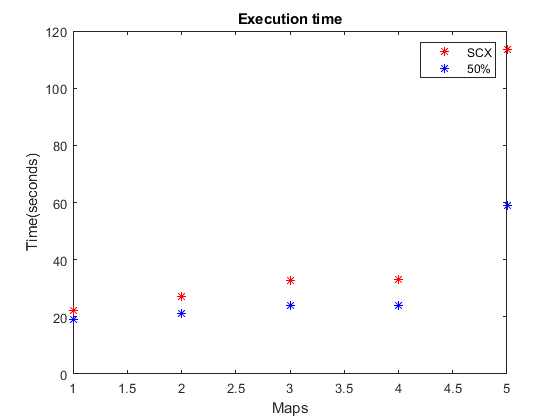
\includegraphics[width=1\textwidth]{tiempo.png}
    \caption{1-eil51 2-eil76 3-kroaA100 4-eil101 5-a280}
\end{figure}

We observe that running time is smaller in the 50\% algorithm. We associate these results to fact that SCX algorithm is more complex. 
It has to search for inside the father like the mother, and if both cities can be inserted, then it calculates the nearly city to the last 
of the child. Also, if we compare the obtained scores

\begin{figure}[H]
    \centering
    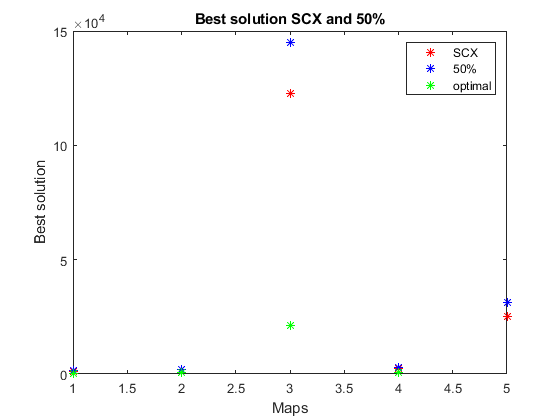
\includegraphics[width=1\textwidth]{solutions.png}
    \caption{1-eil51 2-eil76 3-kroaA100 4-eil101 5-a280}
\end{figure}
We do not have the optimal solution available for the last map, that is why the green asterisk does not appear in the position nº 5. 
As we can observe, the operator SCX obtains better solutions than the 50\% operator. This is due to SCX have into account the 
nearest city with respect to the last city inserted in the child (as the child is being created). However, the 50\% operator only have 
into account if it can add the city or not.

\section{Conclussion}
At operator level, we observe a time-result relation. If we need to find the best solution to these two algorithms, it is worth using SCX 
operator in exchange for spending computer time. Instead if we use the 50\% operator we know the solutions will be worse, but it will consume 
less running time. 

As we can observe, the algorithm results are not close to the optimal solution. However, we calculate in reasonable time a solution for NP-Hard 
algorithm. In my view, it is a great progress now that for many systems (GPS included) it is ideal but not strictly necessary to find the 
optimal solution.


Likewise, although the current order algorithm would not change, it could be improved more the running time if we halt certain algorithm parts, 
for example, producing couples and producing children. Thanks to “paralelización” C++ directives and the increment in the processor nucleus number, 
this option is worth 

\section{Bibliography}
\begin{itemize}
    \item Clever Algorithms Nature-Inspired Programming Recipes, by Jason Brownlee. First Edition. LuLu. January 2011
    \item Comparison of Parents Selection Methods of Genetic Algorithm for TSP. Proceedings published by International Journal of Computer Applications® (IJCA)
    International Conference on Computer Communication and Networks CSI- COMNET-2011
    \item Genetic Algorithm for the Traveling Salesman Problem using Sequential Constructive Crossover Operator. Zakir H. Ahmed zhahmed@gmail.com
    Department of Computer Science, Al-Imam Muhammad Ibn Saud Islamic University,
    \item Genetic Algorithms for the Travelling Salesman Problem: A Review of Representations and Operators. Artificial Intelligence Review
    April 1999, Volume 13, Issue 2, pp 129–170
    \item A Memetic Algorithm with a large neighborhood crossover operator for the Generalized Traveling Salesman Problem. Computers \& Operations Research
    Volume 37, Issue 11, November 2010, Pages 1844-1852
    \item On Solving Travelling Salesman Problems by Genetic Algorithms Heinrich Braun Institut fiir Logik, Komplexitht und Deduktionssysteme, Universi~t Karlsruhe Posffach 6980, 
    D 7500 Karlsruhe, Deutschland, e-maih braun@ira.uka.de
    \item A new crossover approach for solving the multiple travelling salesmen problem using genetic algorithms.
    Shuai Yuan, Bradley Skinner, Shoudong Huang, Dikai Liu. European Journal of Operational Research
    Volume 228, Issue 1, 1 July 2013, Pages 72-82
\end{itemize}
\end{document}